\chapter{Uitwerking IMP} \label{chap:AppendixUitwerkingIMP}
In dit hoofdstuk zal voor de verschillende systemen de automatisering van installatie en configuratie met behulp van IMP uitgelegd worden. Er zal steeds de afhankelijkheden gegeven worden, een domeinmodel, uitleg bij het domeinmodel en voorbeeld configuratie gegeven worden. 

De automatisatie van installatie is ontwikkeld en getest met Fedora 18 en 20, op andere distributies en versies is er niet getest. 
Elk systeem maakt gebruik van \textit{ip::services::Server}, een instantie hiervan is een (virtuele) machine met een IP adres en besturingssysteem. 

Bij elke instantie is het verplicht om de firewall uit te zetten en SELinux op permissive te zetten. Dit kan met behulp van de volgende commando's: 
\begin{lstlisting}[frame=single, breaklines=true]
systemctl stop firewalld.service  
systemctl disable firewalld.service  
setenforce 0
sed -i "s/SELINUX=enforcing/SELINUX=permissive/g" /etc/sysconfig/selinux
sed -i "s/SELINUX=enforcing/SELINUX=permissive/g" /etc/selinux/config|
\end{lstlisting}

\section{HBase}
\textit{Link: \url{https://github.com/thuys/hbase}}

Benodigde IMP modules: std, net, ip, redhat, hosts en yum. 

De installatie en configuratie is gebeurd aan de hand van de uitleg en yum-repository van Cloudera\footnote{\url{http://www.cloudera.com/content/cloudera-content/cloudera-docs/CDH4/4.2.0/CDH4-Installation-Guide/CDH4-Installation-Guide.html}}. 

\subsection{Domein model en uitleg}
Het domeinmodel is te zien in figuur \ref{fig:imp-hbase-domeinmodel}.

\paragraph{HBaseMaster} Dit is de implementatie van de HMaster, dient toegewezen worden aan een host met java installatie. De poort is de poort waarop de HMaster actief is. 
 
\paragraph{HRegion} Dit is de implementatie van de HRegionServer, dient toegewezen worden aan een host met java installatie. De poort is de poort waarop de HRegionServer actief is. 

\paragraph{HadoopHDFS} Dit is de implementatie van de HDFS namenode, dient toegewezen worden aan een host met java installatie. De poort is de poort waarop de namenode actief is, de directory is de directory voor HBase  en de nameDir de lokatie waar de data op harde schijf weggeschreven zal worden. 

\paragraph{HadooDatapHDFS} Dit is de implementatie van de HDFS datanode, dient toegewezen worden aan een host met java installatie. De poort is de poort waarop de namenode datanode is, de directory is de directory voor HBase en de dataDir de lokatie waar de data op harde schijf weggeschreven zal worden. 

\paragraph{Zookeeper} Dit is de implementatie van een enkele Zookeeper. Bij het toewijzen van meerdere aan een cluster zullen de Zookeepers een cluster vormen. 

\paragraph{Javahost} Dit is een server waar Java is op geïnstalleerd. 

\begin{figure}[ht!]
\centering
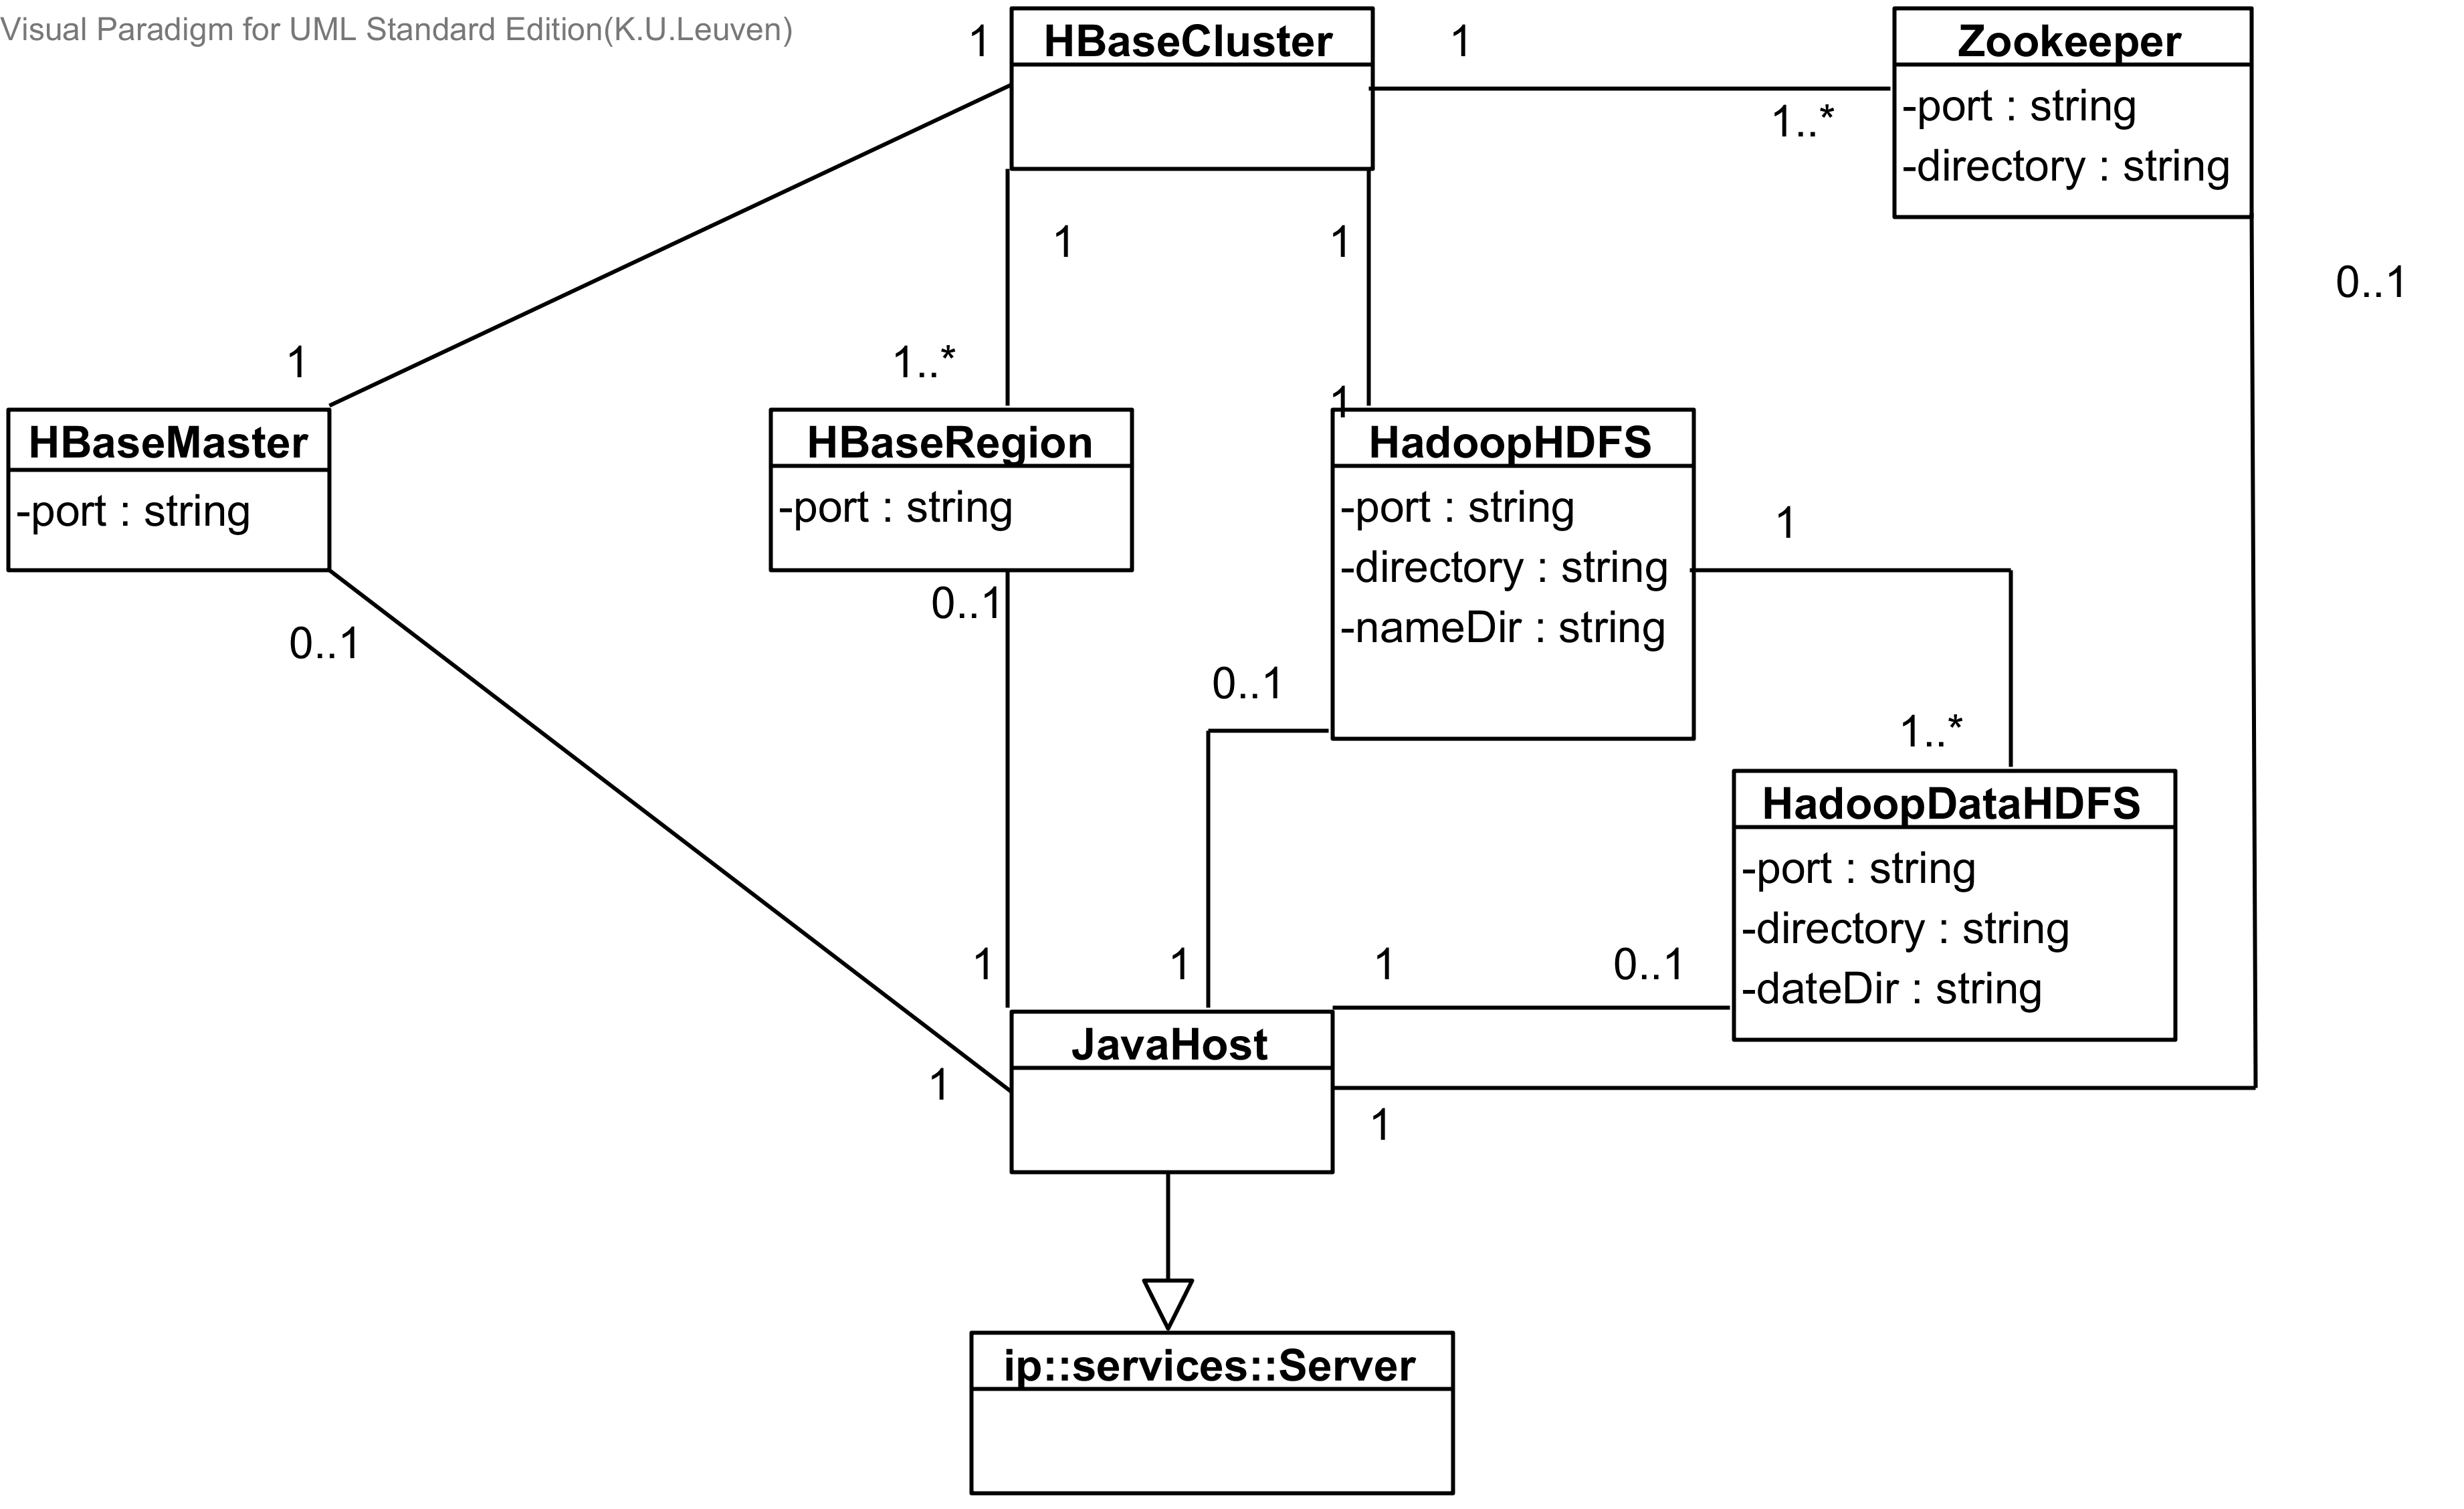
\includegraphics[width=\linewidth]{img/HBase-Domeinmodel.png}
\caption{HBase: Domeinmodel HBase in IMP}
\label{fig:imp-hbase-domeinmodel}
\end{figure}

\subsection{Voorbeeld configuratie}
De configuratie voor de testomgeving gaat als volgt: 

\lstinputlisting[language=Python, breaklines=true, frame=single]{code/imp-hbase.conf}


\section{MongoDB}
\textit{Link: \url{https://github.com/thuys/mongodb}}

Benodigde IMP modules: std, net, ip, redhat, hosts en yum. 

De installatie en configuratie is gebeurd aan de hand van de uitleg en yum-repository van MongoDB\footnote{\url {http://docs.mongodb.org/manual/tutorial/install-mongodb- on-red-hat-centos-or-fedora-linux/}, \url{http://docs.mongodb.org/manual/tutorial/deploy-replica-set-for-testing/} en  \url{http://docs.mongodb.org/manual/tutorial/deploy-shard-cluster/}}. 

\subsection{Domein model en uitleg}
Het domeinmodel is te zien in figuur \ref{fig:imp-mongodb-domeinmodel}.

	\paragraph{MongoDB} is een server in het IMP model en is verantwoordelijk voor het installeren van de basis van MongoDB. Hierna zijn basis commando's voor connectie te maken met een MongoDB instantie beschikbaar. 
	\paragraph{MonogDBServer} is een server in het IMP model en is verantwoordelijk voor het installeren van de MongoDB server. 
	\paragraph{MongoDBNode} is de implementatie van een data instantie, maximaal 1 per server. Indien gelinkt met een replica set zal deze als een deel van een replica set worden geïnitialiseerd, anders als een zelfstandige instantie. 
	\paragraph{MongoDBReplicaSet} is de voorstelling van een replica set, dit wordt niet aan een specifieke server toegewezen. 
	\paragraph{MongoDBReplicaSetController} is verantwoordelijk om de replica set te initialiseren. Belangrijk is dat indien er een uitbreiding is van de set, de node verbonden met de controller een reeds geïnitialiseerde node is.  
	\paragraph{MongoDBConfigServer} is de implementatie van een configuratie server, 1 of 3 servers zijn nodig per cluster. 
	\paragraph{MongoDBAccessServer} is de implementatie van mongos, minstens 1 is nodig maar meer kunnen gebruikt worden.
	\paragraph{MongoDBShardCluster} is de voorstelling van een cluster van shards, er kunnen zowel alleenstaand instanties als replica sets aan toegevoegd worden. 
	\paragraph{MongoDBShardController} is verantwoordelijk om de cluster te initialiseren met de verschillende shards, databases, collecties en keys. 
	\paragraph{MongoDBDatabase} is de voorstelling van een database.
	\paragraph{MongoDBCollection} is de voorstelling van een collectie, indien verbonden met een cluster via een database zal deze gedeeld worden over de verschillende shards. 
	\paragraph{MongoDBKey} is de wijze waarmee een collectie verdeeld wordt over de verschillende shards. 

\begin{figure}[ht!]
\centering
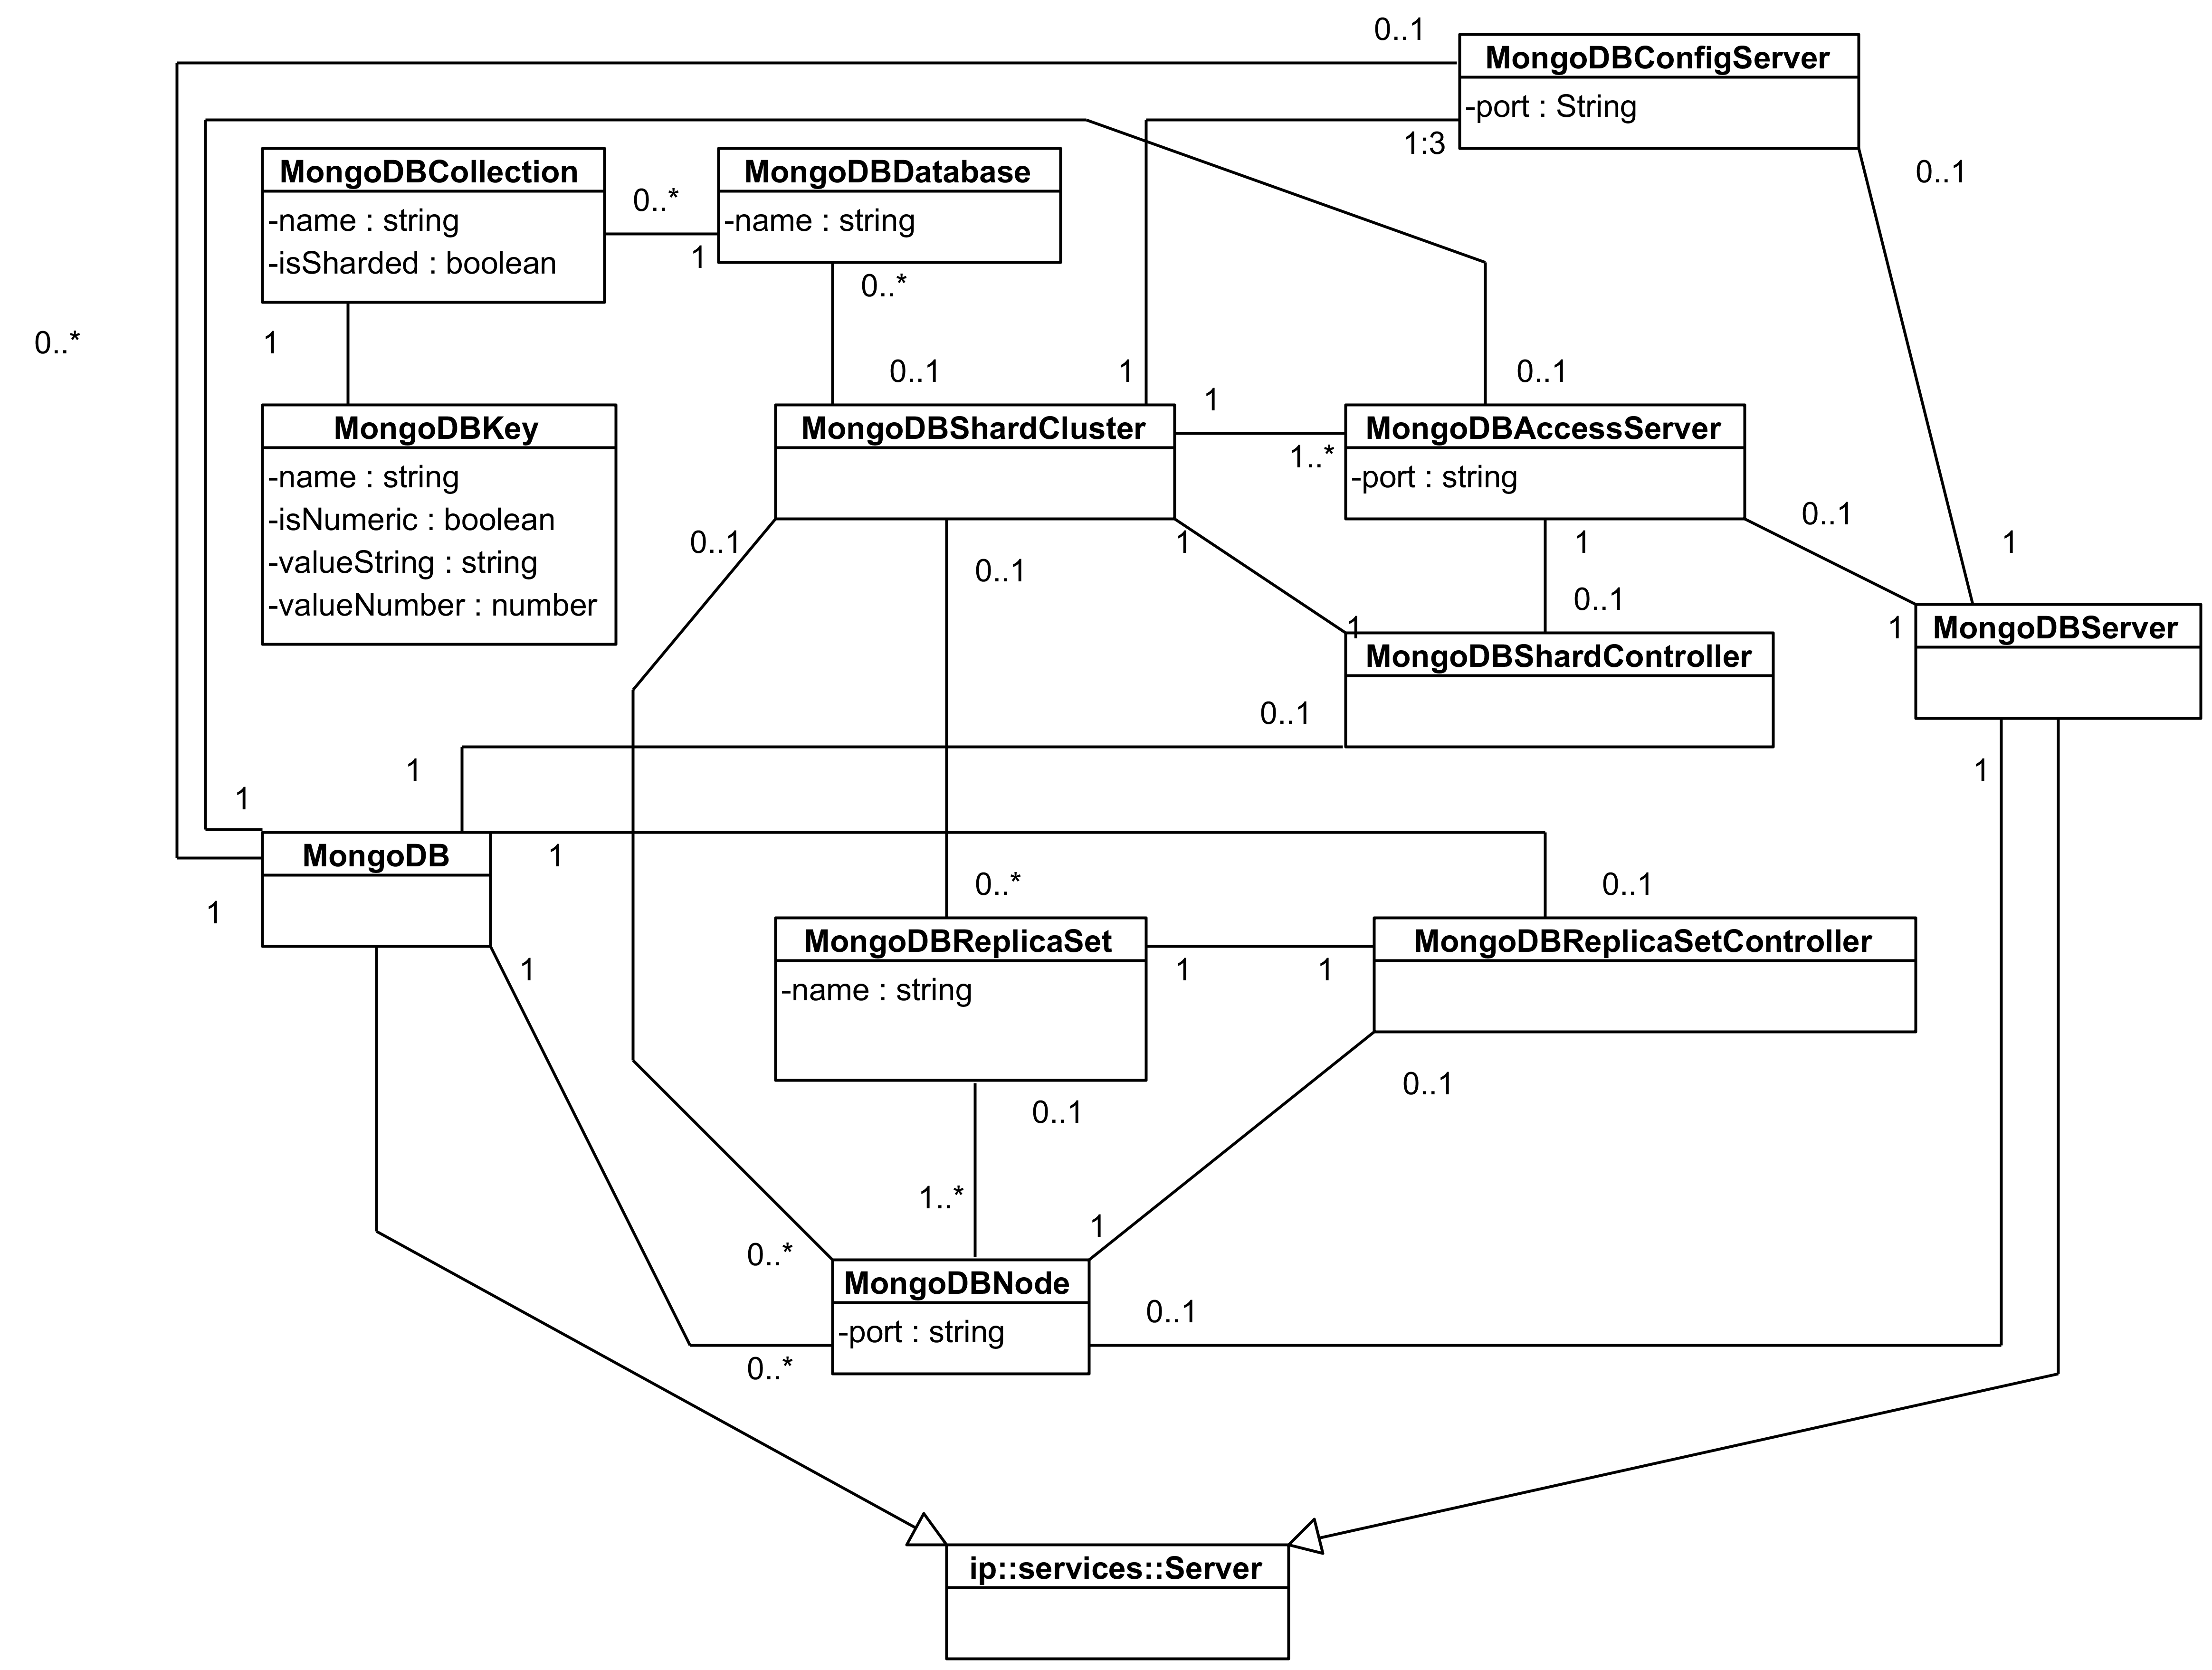
\includegraphics[width=\linewidth]{img/MongoDB-Domeinmodel.png}
\caption{MongoDB: Domeinmodel MongoDB in IMP}
\label{fig:imp-mongodb-domeinmodel}
\end{figure}

\subsection{Voorbeeld configuratie}
De configuratie voor de testomgeving gaat als onderstaand. Bij de uitrol van IMP gaat dit verschillende keren uitgevoerd moeten worden omdat eerst de MongoDBNodes moeten draaien, vervolgens kunnen de replicasets aangemaakt worden, daarna kunnen de replicasets pas toegevoegd worden in de cluster. 

In IMP was het nog niet mogelijk om een te zeggen dat x uitgevoerd moet zijn op een andere instantie, vooraleer y kan uitgevoerd worden, ondertussen is dit mogelijk door de thesis van Harm De Weirdt\cite{thesisHarm} waar de nieuwe installatie beschikbaar is op \url{https://github.com/Foezjie/mongodb} maar hierbij dient ook gebruik gemaakt te worden van zijn IMP installatie.  \\
Met het ontbreken hieraan kan het zijn dat er 3 keer een volledige IMP deploy uitgevoerd moet worden. 

\lstinputlisting[language=Python, breaklines=true, frame=single]{code/imp-mongodb.conf}


\section{Pgpool-II}
\textit{Link: \url{https://github.com/thuys/postgresql}}

Benodigde IMP modules: std, net, ip, redhat, hosts en yum. 

De installatie en configuratie is gebeurd aan de hand van de uitleg Pgpool-II\footnote{\url {http://pgpool.projects.pgfoundry.org/pgpool-II/doc/tutorial-en.html/}}. 

\subsection{Domein model en uitleg}
Het domeinmodel is te zien in figuur \ref{fig:imp-pgpool-domeinmodel}.

	\paragraph{PgpoolMain} Dit is de implementatie van de Pgpool-II router node. 
	
	\paragraph{PgpoolNode} Dit is de implementatie van de Pgpool-II data node die een uitbreiding is van de standaard PostgreSQL installatie. 
		
	\paragraph{PostgresqlServer} Dit is de implementatie van de standalone PostgreSQL server. 

\begin{figure}[ht!]
\centering
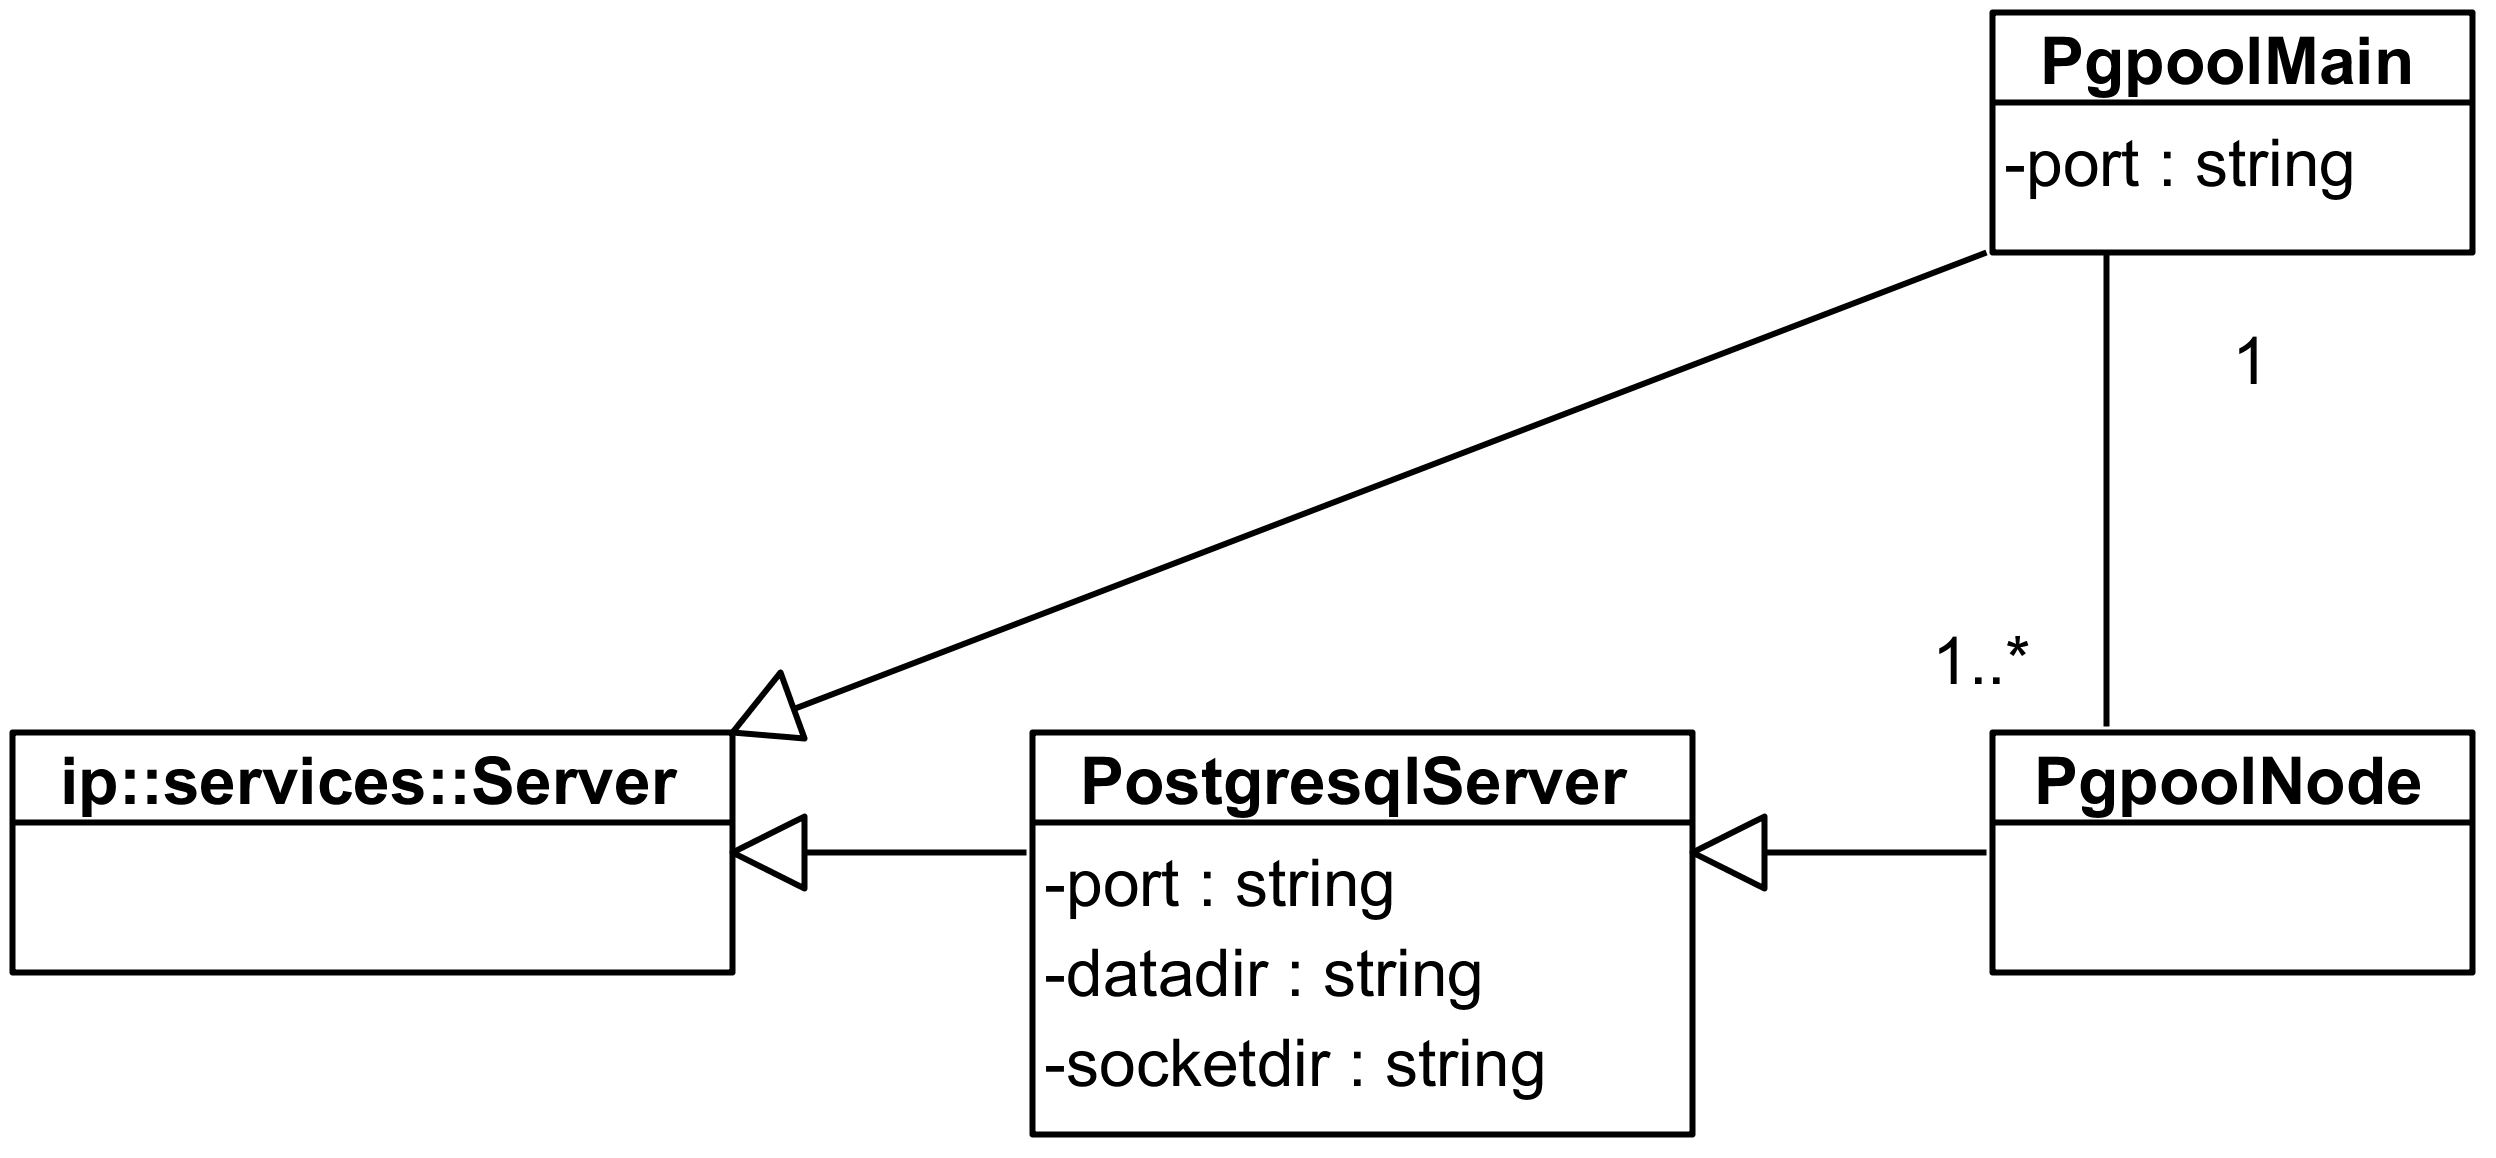
\includegraphics[width=\linewidth]{img/Postgres-Domeinmodel.png}
\caption{Pgpool-II: Domeinmodel Pgpool-II in IMP}
\label{fig:imp-pgpool-domeinmodel}
\end{figure}

\subsection{Voorbeeld configuratie}
De configuratie van Pgpool-II gebeurt in verschillende stappen: shell code, IMP uitrol, extra configuratie stap, IMP uitrol. 

De eerste shell code bestaat erin om de SELinux volledig uit te schakelen: 
\begin{lstlisting}[frame=single, breaklines=true]
systemctl stop firewalld.service  
systemctl disable firewalld.service  
echo "SELINUX=disabled SELINUXTYPE=targeted" > /etc/selinux/config

echo "SELINUX=disabled SELINUXTYPE=targeted" > /etc/sysconfig/selinux
\end{lstlisting}

De configuratie voor de testomgeving gaat als volgt in IMP: 

\lstinputlisting[language=Python, breaklines=true, frame=single]{code/imp-pgpool.conf}

De configuratie bestaat erin om al de verschillende nodes van Pgpool-II, ongeachte of dit routers of datanodes zijn, ssh toegang te geven tot elkaar server via ssh met root en postgres als gebruikers. Deze verbinding al een keer gemaakt zijn want een bericht dat de sleutel nu mee is opgeslagen is voldoende om de online recovery te doen falen. 

Hierna kan de IMP uitrol nog een keer gebeuren en het systeem zou moeten werken. 


\section{YCSB}
\textit{Link: \url{https://github.com/thuys/ycsb}}

Benodigde IMP modules: std, net, ip, redhat, hosts, yum, git, hbase, mongodb, pgpool-II 

De installatie en configuratie is gebeurd aan de hand van de uitleg van YCSB\footnote{\url {https://github.com/brianfrankcooper/YCSB/wiki/}}. 

\subsection{Domein model en uitleg}
Het domeinmodel is te zien in figuur \ref{fig:imp-ycsb-domeinmodel}.
\begin{figure}[ht!]
\centering
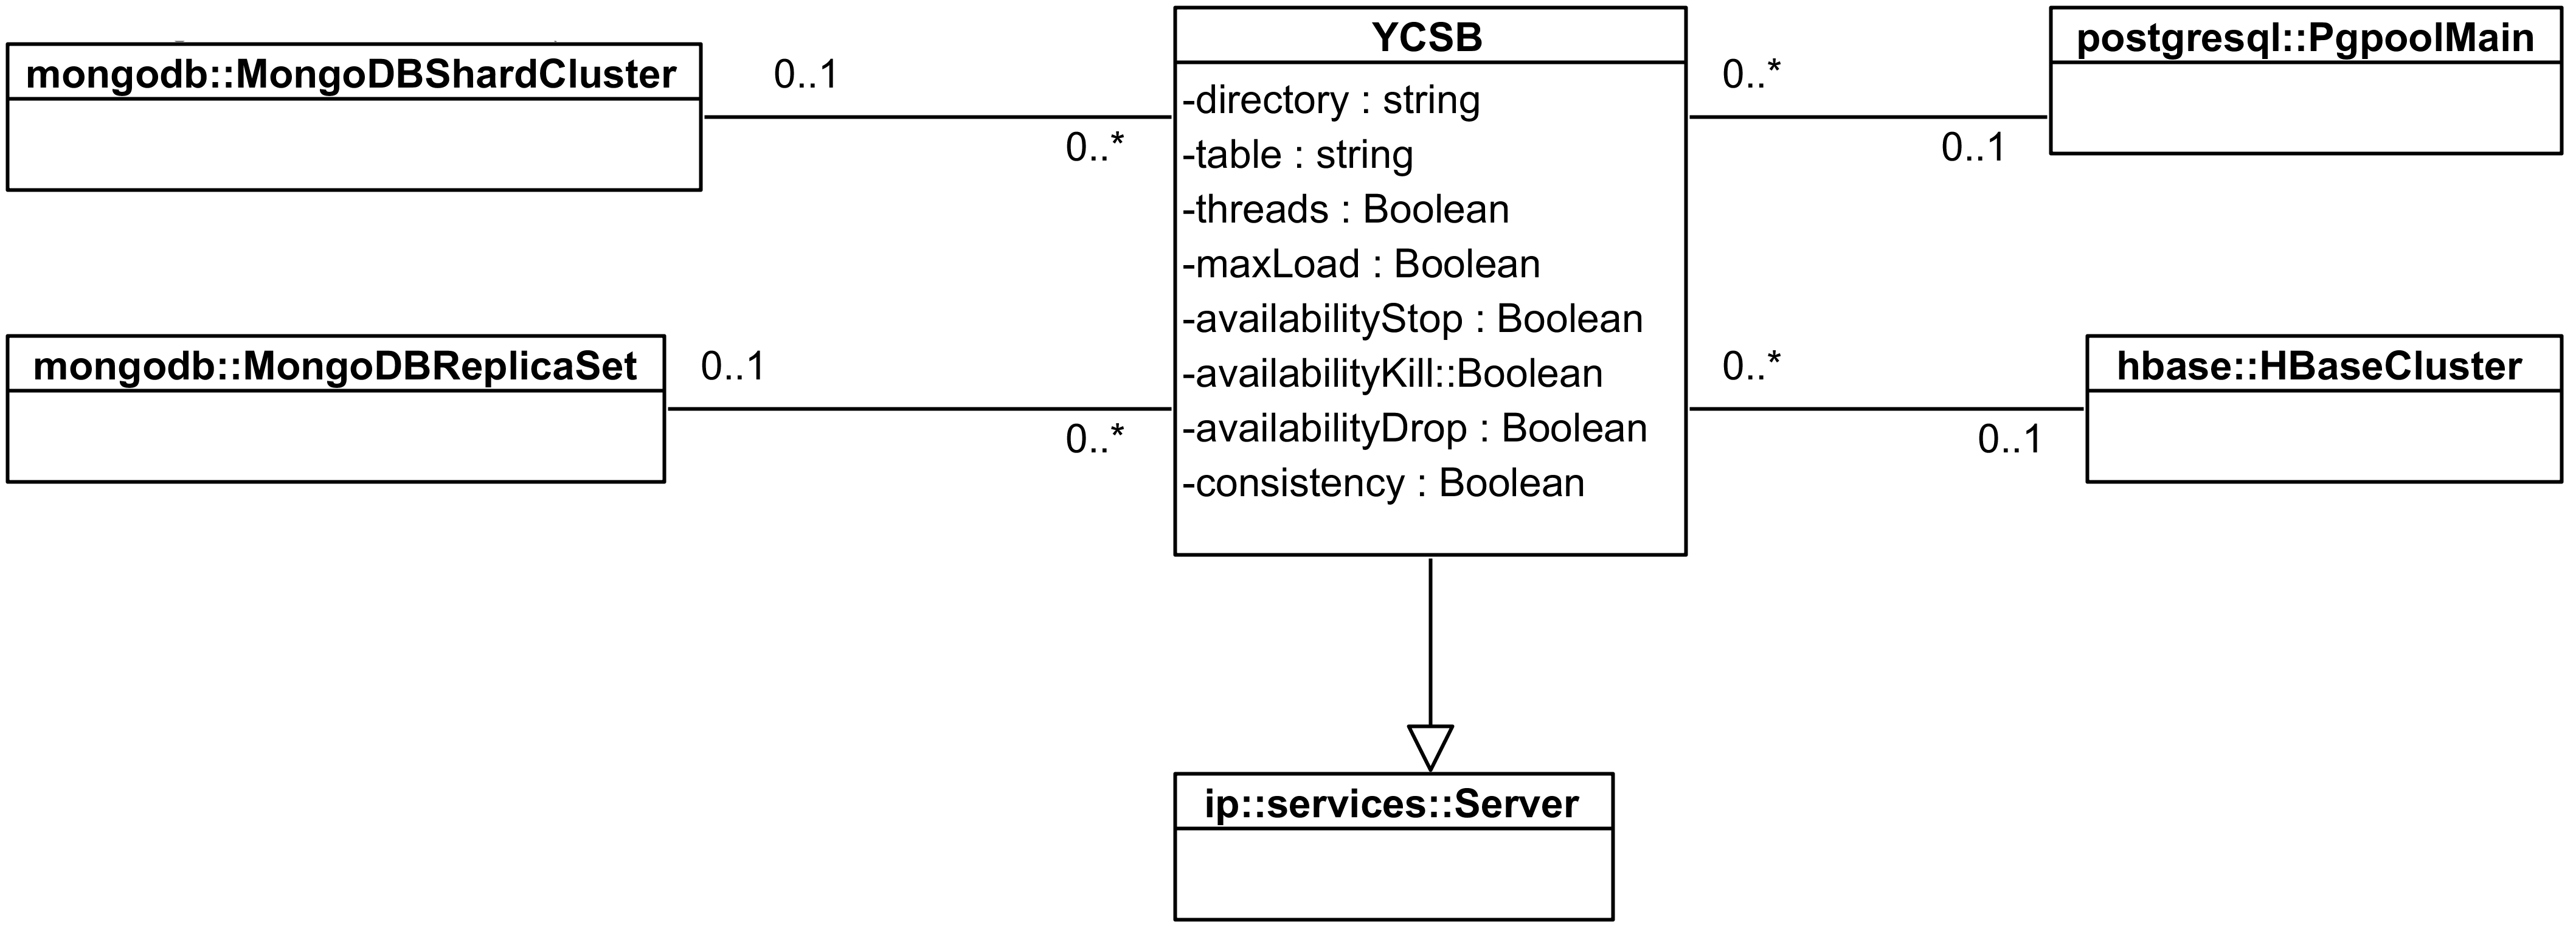
\includegraphics[width=\linewidth]{img/YCSB-Domeinmodel.png}
\caption{YCSB: Domeinmodel YCSB in IMP}
\label{fig:imp-ycsb-domeinmodel}
\end{figure}

Dit model bevat maar 1 nieuw element en dit is YCSB. Deze dient verbonden te zijn met één van de 3 systemen die hierboven zijn beschreven. Elk van deze systemen zal getest worden voor alle testen die geactiveerd zijn. MongoDB heeft 2 connecties omdat de cluster voor de beschikbaarheidstesten wordt gebruikt en een replicaset voor de consistentie testen. Pgpool-II heeft geen ondersteuning voor de consistentie testen. 

\subsection{Voorbeeld configuratie}

De configuratie voor de testomgeving gaat als volgt in IMP: 

\lstinputlisting[language=Python, breaklines=true, frame=single]{code/imp-ycsb.conf}

De testen starten door het uitvoeren van {{directory}}/scripts/ycsb-script. De resultaten komen in de folder {{directory}}/results. 
